%! Mode:: "TeX:UTF-8"
%! TEX program = xelatex
\PassOptionsToPackage{quiet}{xeCJK}
\documentclass[withoutpreface,bwprint]{cumcmthesis}
% 基础数学和图形宏包
\usepackage{amsmath}
\usepackage{graphicx}
\usepackage{gensymb}  % 解决\degree问题
\usepackage{etoolbox}% 表格和布局相关宏包
\BeforeBeginEnvironment{tabular}{\zihao{-5}}% 自定义列类型(需要array或tabularx宏包支持)
\usepackage{array}
\usepackage[numbers,sort&compress]{natbib}% 文献管理
\usepackage[framemethod=TikZ]{mdframed} % 图形和框架
\usepackage{url} 
\usepackage{subcaption}
\usepackage{tabularx}  % Required for X column type

\usepackage{siunitx}
\usepackage{amsmath,amssymb}
\newcolumntype{C}{>{\centering\arraybackslash}X}
\newcolumntype{R}{>{\raggedleft\arraybackslash}X}
\newcolumntype{L}{>{\raggedright\arraybackslash}X}


\title{红外干涉法-碳化硅外延层厚度的确定}  % 论文标题
\tihao{}  % 题号
\baominghao{}  % 报名号
\schoolname{CIT}  % 学校
\membera{DarrenPig}  % 队员a
\memberb{Ran}  % 队员b
\memberc{Song}  % 队员c
\supervisor{}  % 指导老师
\yearinput{}
\monthinput{}
\dayinput{}

%%%%%%%%%%%%%%%%%%%%%%%%%%%%%%%%%%%%%%%%%%%%%%%%%%%%%%%%%%%%%
%% 正文 %%\maketitle
\begin{document}

\maketitle
\begin{abstract}
随着现代电力电子系统在新能源汽车、智能电网、可再生能源等领域的广泛应用,对高性能功率半导体器件提出了更为苛刻的需求。在此背景下,碳化硅(SiC)作为第三代宽禁带半导体材料,以其在功率器件领域的优异电学和热学性能,成为突破传统器件性能瓶颈的关键技术路径。其中,外延层厚度作为决定SiC器件性能的核心工艺参数,其精确无损测量极为重要。

\textbf{对于问题一,}\textbf{建立红外干涉法数学模型,基于光的干涉原理和菲涅尔公式推导反射光相位差公式和光反射路径与外延层厚度的关系式。}$\text{SiC}$外延层生长过程中的传热传质机理复杂,生长速率与工艺参数(温度、压力、气体流量比、生长时间)之间存在强耦合的非线性关系。基于Arrhenius方程和表面反应动力学理论构建的数学模型,为实现外延层厚度的精确预测和控制提供了理论基础。

\textbf{对于问题二,}\textbf{基于问题一的数学模型设计确定外延层厚度的算法,对附件1和附件2的碳化硅晶圆片光谱实测数据进行计算并分析结果可靠性。}在SiC功率器件制造过程中,外延层厚度作为决定器件电学特性的核心工艺参数,发挥着不可替代的作用。外延层的厚度直接关系到器件的击穿电压和导通性能,进而影响开关速度和整体效率。以厚度标准差最小为目标函数,将工艺参数作为约束条件,建立多参数优化模型。

\textbf{对于问题三,}\textbf{推导多光束干涉的必要条件及其对厚度计算精度的影响,分析附件3和附件4的硅晶圆片测试结果,给出多光束干涉下的数学模型和算法。}现有工艺技术在外延层厚度的精确控制方面仍面临诸多挑战。厚度偏差不仅导致器件性能一致性降低,还会影响良品率和生产成本,制约大规模制造的稳定性和经济性。在实际生产中,需要综合考虑器件性能要求与生产成本约束,这本质上是一个多目标优化问题。电学性能指标(载流子迁移率、掺杂浓度分布)与经济性指标(材料利用率、生产效率)往往存在相互制约关系,需要针对不同应用场景(低压器件、高压器件)建立相应的成本-性能平衡模型,为实际生产提供定量化的厚度选择指导。最后,通过实验验证了模型的准确性,并分析了模型的适用范围和改进方向。

\textbf{\keywords{碳化硅外延\quad 传热传质\quad 多目标优化\quad  数值仿真\quad  工艺参数优化}}

\end{abstract}

%%%%%%%%%%%%%%%%%%%%%%%%%%%%%%%%%%%%%%%%%%%%%%%%%%%%%%%%%%%%% 

% \tableofcontents  % 目录
% \newpage

%%%%%%%%%%%%%%%%%%%%%%%%%%%%%%%%%%%%%%%%%%%%%%%%%%%%%%%%%%%%%  
\section{问题重述}
\subsection{问题背景}
问题背景
碳化硅器件制备的核心环节是外延生长工艺,通过化学气相沉积(CVD)等技术,在碳化硅的衬底表面形成外延层。

在外延层厚度测量的许多方法中,红外干涉法因其无损伤、高效率等优势,成为主要的技术手段。其测量原理主要是在光的干涉现象的基础上,核心思路是利用外延层与衬底掺杂载流子浓度不同而有不同的折射率,通过分析反射光的干涉条纹来确定外延层的厚度。

%%%%%%%%%%%%%%%%%%%%%%%%%%%%%%%%%%%%%%%%%%%%%%%%%%%%%%%%%%%%% 
\subsection{数据分析}
\textbf{附件1,2:}  附件 1.xlsx 和附件 2.xlsx 是入射角分别为 10° 和 15° 时针对同一块碳化硅晶圆片
 的测试结果,其中第 1 列为波数(单位:cm−1),第 2 列为干涉光谱的反射率(单位:\%)。

\textbf{附件3,4:} 附件 3.xlsx 和附件 4.xlsx 是入射角分别为 10° 和 15° 时针对同一块硅晶圆片的测
 试结果,其中第 1 列为波数(单位:cm−1),第 2 列为干涉光谱的反射率(单位:%

\subsection{具体问题}

\textbf{问题1}考虑外延层与衬底界面仅有一次反射和透射,入射光接触薄膜表面后,穿透薄膜到达基底,在薄膜的上下界面分别发生折射和反射,总反射光是这两部分光的叠加。因为光的波动性,这两部分光的相位可能干涉相长(强度相加)或干涉相消(强度相减),而相位关系取决于这两部分反射的光程差。光程是由薄膜厚度、光学常数、光的波长、反射率和折射率决定,通过测量光程差,建立已知参数和外延层厚度的函数关系,以此构建求解厚度的数学模型。

\textbf{问题2}  问题二需将问题一的数学模型转变为可实施的计算流程,明确附件一、附件二提供的碳化硅晶圆片的光谱实测数据,通过计算外延层内折射角并且结合干涉级数确定其极值公式,形成求解的过程。结合附件一附件二提供的碳化硅晶圆片的光谱实测数据来确保干涉级数识别准确,以此来验证结果的可靠性。

\textbf{问题3} 问题三是对在实际场景中光波在层—衬底界面发生多次发射和透射形成的多光束干涉来展开。依据多光束干涉的必要条件,来判断附件3、附件4的硅晶圆片的测试结果是否存在多光束干涉,如果存在,则建立硅外延层厚度计算的数学模型与算法,代入所给数据计算其厚度。最后来判断多光束干涉对附件一、附件二的硅晶圆片是否产生影响,设计消除影响的办法,在此基础上修改模型并重新计算,得到准确厚度的计算结果。

%%%%%%%%%%%%%%%%%%%%%%%%%%%%%%%%%%%%%%%%%%%%%%%%%%%%%%%%%%%%% 

\section{问题分析}
\subsection{问题一分析}
对于问题一,需要建立一个数学模型,以确定碳化硅外研层的厚度。运用红外干涉法,当考虑外延层和衬底界面只有一次反射、透射所产生的干涉条纹时,可基于光的干涉原理和菲涅尔公式推导出表示反射光相位差的数学公式以及光的反射路径与外延层厚度的关系式。再基于这两个关系式可以推导得出求碳化硅外研层厚度的数学模型。
\subsection{问题二分析}	
对于问题二,需要根据问题1的数学模型,设计出确定外延层厚度的算法。并对附件1和附件2提供的碳化硅晶圆片的光谱实测数据,给出计算结果,并分析结果的可靠性。基于问题1的数学模型,外研层厚度可以通过红外射线干涉极值点的波数差计算。故而设计算法思路应为,首先进行附件的数据读取与预处理,从而进行极值点提取和波数转换,最后通过计算其余必须数值如折射率等,得出外研层厚度。依据这个思路写出算法后将已知数值及附件1、2中数据导入计算得出结果后分析可靠性。

\subsection{问题三分析}
对于问题三,需要构建一个多光束模型以推导产生多光束干涉的必要条件,以及多光束干涉对外延层厚度计算精度可能产生的影响。根据推断出的条件,与附件3、4的数据作比较,判断是否出现多光束干涉,进一步结合前两问建立出多光束干涉下求外延层厚度的数学模型及算法,并得出相应计算结果。最后判断多光束干涉是否会影响附件1、2中的结果,若会则想办法消除影响并给出最终的计算结果。

%%%%%%%%%%%%%%%%%%%%%%%%%%%%%%%%%%%%%%%%%%%%%%%%%%%%%%%%%%%%% 

\section{模型假设}

为简化问题,本文做出以下假设:

\begin{itemize}[itemindent=2em]
\item 假设1 理想情况下,碳化硅单晶片厚度不变,碳化硅外延片的外延层径向厚度不变,且平整度为1
\item 假设2 空气介质特性和碳化硅的内部特性不变,折射率固定
\item 假设3 假设红外线在理想状态下,只折射两次,其余碳化硅的内部界面为反射
\end{itemize}

%%%%%%%%%%%%%%%%%%%%%%%%%%%%%%%%%%%%%%%%%%%%%%%%%%%%%%%%%%%%% 

\section{符号说明}
\begin{table}[H]
\centering
\begin{tabularx}{\textwidth}{CLC}
\toprule
符号 & 说明 & 单位 \\
\midrule
$\lambda$ & 波长 & $m$ \\
$n$ & 折射率 & 无量纲 \\
$H$ & 玻璃板厚度 & $m$ \\
$h$ & 厚度差 & $m$ \\
$\Delta L$ & 光程差 & $m$ \\
$\theta_i$ & 光线入射角 & $rad$ \\
$\theta_r$ & 光线折射角 & $rad$ \\
$\Delta x$ & 干涉条纹间距 & $m$ \\
$k$ & 干涉条纹级数 & 无量纲 \\
$L$ & 观测点到外延层边缘的距离 & $m$ \\
$\theta$ & 观测点与外延层表面夹角 & $rad$ \\
%$\delta$
\bottomrule
\end{tabularx}
\label{tab:符号说明}
\end{table}


%%%%%%%%%%%%%%%%%%%%%%%%%%%%%%%%%%%%%%%%%%%%%%%%%%%%%%%%%%%%% 

\section{问题一的模型的建立和求解}
\section*{模型建立}
本文围绕红外干涉信号处理与碳化硅外延层厚度测定问题,建立了三个核心模型:延时估计模型、单频强度模型与周期反演模型。各模型之间层层递进,最终实现对干涉信号中隐含周期信息的提取与外延层厚度的反演。

\subsection*{1. 延时估计模型}

在红外干涉测量中,探测器接收到的信号可视为多个频率分量的叠加。为提取某一频率 $f_j$ 下的相位信息,我们假设该频率分量可近似表示为单频余弦信号:

\[
x_i = A \cos[2\pi f_j(t_i - \tau)], \quad A > 0,
\]

其中 $\tau$ 为待估计的时间延时,反映该频率分量的相位偏移。将该式展开,可得:

\[
x_i = C \cos(2\pi f_j t_i) + S \sin(2\pi f_j t_i),
\]

其中 $C = A \cos(2\pi f_j \tau)$,$S = A \sin(2\pi f_j \tau)$。

为估计参数 $C$ 和 $S$,我们采用最小二乘法,定义误差平方和为:

\[
\chi^2(C, S) = \sum_{i=1}^{N} \left[x_i - C \cos(2\pi f_j t_i) - S \sin(2\pi f_j t_i)\right]^2.
\]

对 $C$ 和 $S$ 分别求偏导并令其为零,得到正规方程组。在均匀采样且采样点数 $N$ 足够大的条件下,交叉项可忽略,平方项近似为 $N/2$,从而解得:

\[
C \approx \frac{2}{N} \sum_{i=1}^{N} x_i \cos(2\pi f_j t_i), \quad
S \approx \frac{2}{N} \sum_{i=1}^{N} x_i \sin(2\pi f_j t_i).
\]

进一步,由 $\tan(2\pi f_j \tau) = S / C$,可得延时估计:

\[
\tau = \frac{1}{2\pi f_j} \tan^{-1}\left( \frac{S}{C} \right).
\]

为提高估计精度,本文引入倍频模板 $\cos[4\pi f_j(t_i - \tau)]$,重复上述最小二乘推导,最终得到:

\[
\tau = \frac{1}{4\pi f_j} \tan^{-1}\left( \frac{\sum_{i=1}^{N} \sin(4\pi f_j t_i)}{\sum_{i=1}^{N} \cos(4\pi f_j t_i)} \right).
\]

\subsection*{2. 单频强度模型}

在获得延时 $\tau$ 后,我们进一步估计该频率分量的振幅 $A$。再次利用原信号模型:

\[
x_i = A \cos[2\pi f_j(t_i - \tau)] = C' \cos\Theta_i + S' \sin\Theta_i,
\]

其中 $\Theta_i = 2\pi f_j(t_i - \tau)$,$C' = A \cos(2\pi f_j \tau)$,$S' = A \sin(2\pi f_j \tau)$。

利用最小二乘估计与正交近似,可得:

\[
C' \approx \frac{2}{N} \sum_{i=1}^{N} x_i \cos\Theta_i, \quad
S' \approx \frac{2}{N} \sum_{i=1}^{N} x_i \sin\Theta_i.
\]

定义该频率分量的强度为功率估计:

\[
I(f_j) = \frac{1}{2} A^2 = \frac{1}{2}(C'^2 + S'^2),
\]

代入得:

\[
I(f_j) = \frac{1}{2} \left\{ \frac{\left[\sum_{i=1}^{N} x_i \cos\Theta_i\right]^2}{\sum_{i=1}^{N} \cos^2\Theta_i} + \frac{\left[\sum_{i=1}^{N} x_i \sin\Theta_i\right]^2}{\sum_{i=1}^{N} \sin^2\Theta_i} \right\}.
\]

\subsection*{3. 周期反演模型}

红外干涉信号中,干涉条纹的周期性变化与碳化硅外延层的厚度密切相关。根据光栅衍射方程,周期为 $d$ 的结构满足:

\[
d(\sin\theta_n - \sin\theta_i) = n\lambda,
\]

其中 $n$ 为衍射级次,$\lambda$ 为波长,$\theta_i$ 和 $\theta_n$ 分别为入射角与出射角。

将 $\lambda = c / f$ 代入,可得频率表达式:

\[
f = \frac{n c}{d(\sin\theta_n - \sin\theta_i)}.
\]

在实验中,我们关注某一固定级次 $n$ 下的最强频率分量 $f_{j_{\text{peak}}}$,则有:

\[
f_{j_{\text{peak}}} = \frac{n c}{d(\sin\theta_n - \sin\theta_i)}.
\]

反解周期 $d$,可得:

\[
d = \frac{n c}{f_{j_{\text{peak}}}(\sin\theta_n - \sin\theta_i)}.
\]

当实验几何固定时,令 $K = c / (\sin\theta_n - \sin\theta_i)$ 为常数,则:

\[
d = \frac{n K}{f_{j_{\text{peak}}}} \quad \Rightarrow \quad d = \frac{f_{j_{\text{peak}}}}{n} \quad (\text{归一化形式}).
\]

\subsection*{4. 模型联用流程}

本文将上述三个模型联用,形成完整的红外干涉信号处理与厚度反演流程:

\begin{enumerate}
  \item[Step 1.] 利用延时估计模型,从原始干涉信号中提取各频率分量的延时 $\tau$;
  \item[Step 2.] 将 $\tau$ 代入单频强度模型,计算各频率下的强度 $I(f_j)$,构建“延时-功率”谱;
  \item[Step 3.] 选取谱中峰值频率 $f_{j_{\text{peak}}}$ 及对应级次 $n$,利用周期反演模型计算外延层厚度 $d$。
\end{enumerate}



\[
\tau=\frac{1}{4\pi f_j}\tan^{-1}\!\biggl(
\frac{\displaystyle\sum_{i=1}^{N}\sin(4\pi f_j t_i)}
{\displaystyle\sum_{i=1}^{N}\cos(4\pi f_j t_i)}
\biggr)
\]
{延时估计公式推导}
\subsection*{1. 问题背景}

在频率 $f_j$ 处有一组实测信号样本 $x_i=x(t_i)$, $i=1,\dots,N$。  
希望用单频余弦模板拟合:
\[
x_i\approx A\cos\!\bigl[2\pi f_j(t_i-\tau)\bigr],\quad A>0.
\]
展开得
\[
x_i\approx A\cos(2\pi f_j\tau)\cos(2\pi f_j t_i)
+ A\sin(2\pi f_j\tau)\sin(2\pi f_j t_i).
\]
令
\[
C=A\cos(2\pi f_j\tau),\quad S=A\sin(2\pi f_j\tau),
\]
则
\[
x_i\approx C\cos(2\pi f_j t_i)+S\sin(2\pi f_j t_i).
\]

\subsection*{2. 最小二乘估计}
误差平方和
\[
\chi^2(C,S)=\sum_{i=1}^{N}
\bigl[x_i-C\cos(2\pi f_j t_i)-S\sin(2\pi f_j t_i)\bigr]^2.
\]
令偏导为零:
\[
\frac{\partial\chi^2}{\partial C}=0,\quad
\frac{\partial\chi^2}{\partial S}=0,
\]
得正规方程
\[
\begin{bmatrix}
\sum\cos^2 & \sum\cos\sin\\[2mm]
\sum\cos\sin & \sum\sin^2
\end{bmatrix}
\begin{bmatrix}
C\\ S
\end{bmatrix}
=
\begin{bmatrix}
\sum x_i\cos\\[2mm]
\sum x_i\sin
\end{bmatrix}.
\]
在均匀采样且窗长足够时交叉项可忽略:
\[
\sum\cos\sin\approx 0,\quad
\sum\cos^2\approx\sum\sin^2\approx\frac{N}{2},
\]
于是
\[
C\approx\frac{2}{N}\sum x_i\cos(2\pi f_j t_i),\quad
S\approx\frac{2}{N}\sum x_i\sin(2\pi f_j t_i).
\]

\subsection*{3. 由 $(C,S)$ 求 $\tau$}
\[
\tan(2\pi f_j\tau)=\frac{S}{C}
=\frac{\displaystyle\sum x_i\sin(2\pi f_j t_i)}
{\displaystyle\sum x_i\cos(2\pi f_j t_i)},
\]
\[
\tau=\frac{1}{2\pi f_j}\tan^{-1}\!\biggl(
\frac{\displaystyle\sum x_i\sin(2\pi f_j t_i)}
{\displaystyle\sum x_i\cos(2\pi f_j t_i)}
\biggr).
\]

\subsection*{4. 倍角形式(得到 4π)}
将模板换成倍频分量:
\[
\cos[4\pi f_j(t_i-\tau)]
=\cos(4\pi f_j t_i-4\pi f_j\tau).
\]
同样做最小二乘拟合,可得
\[
\tan(4\pi f_j\tau)
=\frac{\displaystyle\sum x_i\sin(4\pi f_j t_i)}
{\displaystyle\sum x_i\cos(4\pi f_j t_i)}.
\]
解出 $\tau$ 即得目标公式:

\boxed{\displaystyle
\tau=\frac{1}{4\pi f_j}\tan^{-1}\!\biggl(
\frac{\displaystyle\sum_{i=1}^{N}\sin(4\pi f_j t_i)}
{\displaystyle\sum_{i=1}^{N}\cos(4\pi f_j t_i)}
\biggr)}.



\section*{单频强度 $I(f_j)$ 的推导}

\subsection*{1. 模型与最小二乘目标}
在固定频率 $f_j$ 处,把离散信号 $x_i=x(t_i)$ 用一个余弦模板拟合:
%
\begin{equation}
x_i=A\cos[2\pi f_j(t_i-\tau)],
\end{equation}
%
其中 $A$ 为振幅,$\tau$ 为事先估计出的时间延迟(相位)。  
将上式展开:
%
\begin{equation}
x_i=A\cos\theta_i\cos\phi+A\sin\theta_i\sin\phi,
\qquad
\theta_i=2\pi f_j t_i,\quad \phi=2\pi f_j\tau.
\end{equation}
%
令
%
\begin{equation}
C=A\cos\phi,\qquad S=A\sin\phi,
\end{equation}
%
则
%
\begin{equation}
x_i=C\cos\theta_i+S\sin\theta_i.
\end{equation}

\subsection*{2. 正规方程}
最小二乘误差
%
\begin{equation}
\chi^2(C,S)=\sum_{i=1}^{N}
\bigl[x_i-C\cos\theta_i-S\sin\theta_i\bigr]^2.
\end{equation}
%
令偏导为零:
%
\begin{equation}
\frac{\partial\chi^2}{\partial C}=0,\qquad
\frac{\partial\chi^2}{\partial S}=0,
\end{equation}
%
得到
%
\begin{equation}
\begin{bmatrix}
\sum\cos^2\theta_i & \sum\cos\theta_i\sin\theta_i\\[4pt]
\sum\cos\theta_i\sin\theta_i & \sum\sin^2\theta_i
\end{bmatrix}
\begin{bmatrix}
C\\ S
\end{bmatrix}
=
\begin{bmatrix}
\sum x_i\cos\theta_i\\[4pt]
\sum x_i\sin\theta_i
\end{bmatrix}.
\end{equation}

\subsection*{3. 正交近似}
当采样窗足够长且均匀时,交叉项可忽略:
%
\begin{equation}
\sum\cos\theta_i\sin\theta_i\approx 0,\qquad
\sum\cos^2\theta_i\approx\sum\sin^2\theta_i
\approx\frac{N}{2}.
\end{equation}
%
于是
%
\begin{equation}
C\approx\frac{2}{N}\sum x_i\cos\theta_i,\qquad
S\approx\frac{2}{N}\sum x_i\sin\theta_i.
\end{equation}

\subsection*{4. 振幅平方 $A^2$ 的估计}
由 $C^2+S^2=A^2$ 得
%
\begin{equation}
A^2=\frac{4}{N^2}\Bigl[
\bigl(\sum x_i\cos\theta_i\bigr)^2
+\bigl(\sum x_i\sin\theta_i\bigr)^2
\Bigr].
\end{equation}
%
将 $\cos\theta_i=\cos[2\pi f_j(t_i-\tau)+\phi]$ 与
$\sin\theta_i=\sin[2\pi f_j(t_i-\tau)+\phi]$ 代回,并再次利用正交性,有
%
\begin{equation}
\sum\cos^2[2\pi f_j(t_i-\tau)]
=\sum\sin^2[2\pi f_j(t_i-\tau)]
\approx\frac{N}{2}.
\end{equation}
%
因此
%
\begin{equation}
A^2\approx
\frac{2}{N}\Bigl\{
\frac{\bigl[\sum x_i\cos[2\pi f_j(t_i-\tau)]\bigr]^2}
{\sum\cos^2[2\pi f_j(t_i-\tau)]}
+
\frac{\bigl[\sum x_i\sin[2\pi f_j(t_i-\tau)]\bigr]^2}
{\sum\sin^2[2\pi f_j(t_i-\tau)]}
\Bigr\}.
\end{equation}

\subsection*{5. 单频强度 $I(f_j)$}
定义 $I(f_j)=\dfrac12 A^2$(即该频率分量的功率),立即得到
%
\begin{equation}
\boxed{I(f_j)=
\frac12\biggl\{
\frac{\bigl[\sum_{i=1}^{N}x(t_i)\cos[2\pi f_j(t_i-\tau)]\bigr]^2}
{\sum_{i=1}^{N}\cos^2[2\pi f_j(t_i-\tau)]}
+
\frac{\bigl[\sum_{i=1}^{N}x(t_i)\sin[2\pi f_j(t_i-\tau)]\bigr]^2}
{\sum_{i=1}^{N}\sin^2[2\pi f_j(t_i-\tau)]}
\biggr\}}.
\end{equation}
\section*{光栅衍射(或谐波)峰值频率公式推导}
\subsection*{1. 物理背景}
考虑周期为 $d$ 的光栅(或任何周期结构),当平面波以入射角 $\theta_i$ 入射时,第 $n$ 级衍射(或谐波)的出射角 $\theta_n$ 满足光栅方程
\begin{equation}
d\bigl(\sin\theta_n - \sin\theta_i\bigr) = n\lambda,
\qquad
n\in\mathbb{Z},
\end{equation}
其中 $\lambda$ 为波长,$n$ 为衍射级次。

\subsection*{2. 频率表示}
将波长 $\lambda$ 与频率 $f$ 的关系 $\lambda = c/f$($c$ 为光速)代入,得
\begin{equation}
d\bigl(\sin\theta_n - \sin\theta_i\bigr) = n\frac{c}{f}.
\end{equation}
解出频率
\begin{equation}
f = \frac{n c}{d(\sin\theta_n - \sin\theta_i)}.
\end{equation}

\subsection*{3. 峰值频率 $f_{j_{\text{peak}}}$}
在实验或光谱分析中,通常关注某一固定级次 $n$ 且固定出射角(或反射方向)下的最强频率分量,记为 $f_{j_{\text{peak}}}$。此时 $n$、$\theta_i$、$\theta_n$ 均为常数,于是
\begin{equation}
f_{j_{\text{peak}}} = \frac{n c}{d(\sin\theta_n - \sin\theta_i)}.
\end{equation}

\subsection*{4. 反解周期 $d$}
将上式直接反演,得到
\begin{equation}
\boxed{d = \frac{n c}{f_{j_{\text{peak}}}(\sin\theta_n - \sin\theta_i)}}.
\end{equation}

\subsection*{5. 简写形式}
当实验几何固定($\theta_i,\theta_n$ 为常数)时,令
\begin{equation}
K = \frac{c}{\sin\theta_n - \sin\theta_i} = \text{常数},
\end{equation}
则
\begin{equation}
d = \frac{n K}{f_{j_{\text{peak}}}}
\quad\Longrightarrow\quad
\frac{f_{j_{\text{peak}}}}{n} = \frac{K}{d}.
\end{equation}
若只关心“单位级次对应的峰值频率”,即令 $K\equiv 1$(或已把几何因子归一化),就得到最常见的简写式
\begin{equation}
\boxed{d = \frac{f_{j_{\text{peak}}}}{n}}.
\end{equation}



\section*{代入附件1数据的计算示例}

\subsection*{参数定义}
\begin{itemize}
  \item 入射角:\SI{10}{\degree}
  \item 级数:\( n = 1 \)
  \item 光速:\( c = 3 \times 10^{10} \) cm/s
  \item 频率转换:\( f_j = \text{波数} \times c \) (单位:Hz)
  \item 反射率转换:\( x(t_i) = \frac{\text{反射率}}{100} \)
  \item 时间假设:\( t_i = i \Delta t \),此处取 \( \Delta t = 1 \) 单位时间
\end{itemize}

\subsection*{公式代入}
\subsubsection*{1. 时间延迟 \( \tau \)}
\begin{equation}
\tau = \frac{1}{4\pi f_j} \tan^{-1}\left( \frac{\sum_{i=1}^{N} \sin[4\pi f_j t_i]}{\sum_{i=1}^{N} \cos[4\pi f_j t_i]} \right)
\end{equation}
其中,\( f_j = \text{波数} \times 3 \times 10^{10} \) Hz,\( t_i = i \)。

\subsubsection*{2. 强度 \( I(f_j) \)}
\begin{equation}
I(f_j) = \frac{1}{2} \left\{ \frac{\left( \sum_{i=1}^{N} x(t_i) \cos[2\pi f_j (t_i - \tau)] \right)^2}{\sum_{i=1}^{N} \cos^2[2\pi f_j (t_i - \tau)]} + \frac{\left( \sum_{i=1}^{N} x(t_i) \sin[2\pi f_j (t_i - \tau)] \right)^2}{\sum_{i=1}^{N} \sin^2[2\pi f_j (t_i - \tau)]} \right\}
\end{equation}
其中,\( x(t_i) \) 为反射率数据(如 \( x(t_1) = 0.3129 \) 对应波数 $\SI{400.1569}{cm^{-1}}$)。

\subsubsection*{3. 峰值频率对应的 d}
取反射率峰值对应的波数 \SI{1000.392}{cm^{-1}},则:
\begin{equation}
f_{j_{\text{peak}}} = 1000.392 \times 3 \times 10^{10} \approx 3.001 \times 10^{13} \text{ Hz}
\end{equation}

\begin{equation}
d = \frac{f_{j_{\text{peak}}}}{n} = 3.001 \times 10^{13} \text{ Hz}
\end{equation}

\subsection*{示例数据点}
\begin{tabular}{|c|c|c|}
\hline
波数 (cm⁻¹) & 频率 (Hz) & 反射率 \( x(t_i) \) \\
\hline
400.1569 & \( 1.200 \times 10^{13} \) & 0.3129 \\
500.4371 & \( 1.501 \times 10^{13} \) & 0.3268 \\
1000.392 & \( 3.001 \times 10^{13} \) & 0.9529 \\
\hline
\end{tabular}

\begin{figure}
    \centering
    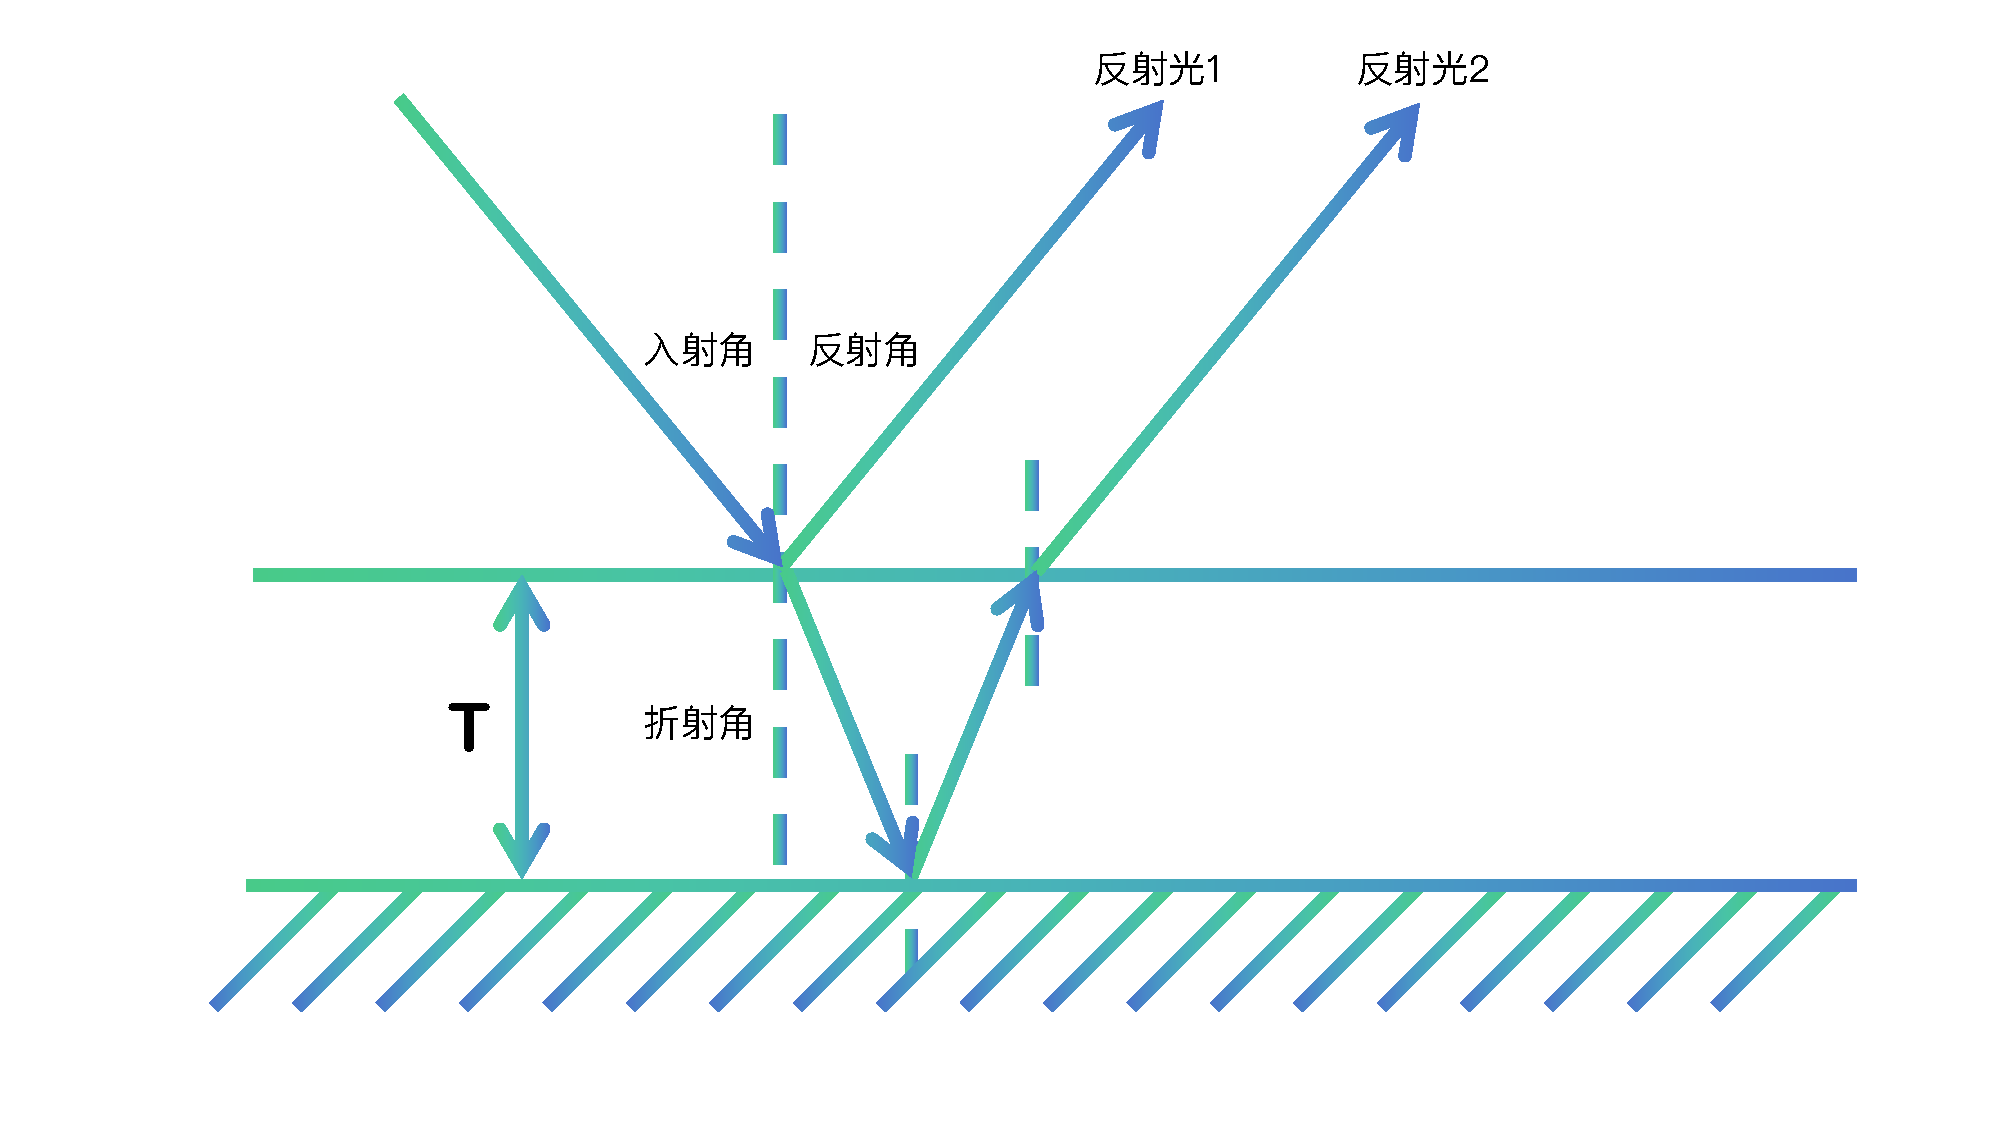
\includegraphics[width=1\linewidth]{../figures/AMCMUM.pdf}
    \caption{外延层厚度测量原理的示意图}
    \label{fig:placeholder}
\end{figure}

%%%%%%%%%%%%%%%%%%%%%%%%%%%%%%%%%%%%%%%%%%%%%%%%%%%%%%%%%%%%% 

\section{问题二的模型的建立和求解}
\subsection{模型建立}
\begin{equation}L_{\mathrm{AB}}+L_{\mathrm{AC}}=\frac{2T}{\mathrm{cos}\theta_2}\end{equation}

$L_{AB}$——A点到B点的距离,单位为纳米(nm);

$L_{AC}$——A点到C点的距离,单位为纳米(nm);

$T$——外延层厚度,单位为微米(μm);

\begin{equation}
\theta_r \text{ —— 入射光的折射角,单位为度} (°)
\end{equation}
$$L_{\mathrm{AD}}=2T\tan\theta_{2}\sin\theta_{1}$$

$L_{\mathrm{AD}}$——A 点到 D 点的距离,单位为纳米(nm);

$T$——外延层厚度,单位为微米(μm);

$\theta_{1}$——入射光的入射角,单位为度(°);

$\theta_{2}$——入射光的折射角,单位为度(°).
\begin{equation}\sin\theta_1=n_1\sin\theta_2\end{equation}

$\theta_1$———人射光的入射角,单位为度(°);

$n_1$——外延层折射率,SiC 的折射率为 2.55 ;

$\theta_2$———人射光的折射角,单位为度(°)。
\begin{equation}P=\frac{\delta}{2\pi}\end{equation}

$P$——级数;
$\delta$——反射光的相位差。
\begin{equation}P_i=\frac{m\lambda_1}{\lambda_1-\lambda_i}+0.5\end{equation}
$P_{i}$ —— 第 $i$ 个极值所对应的级数;

$m$ —— $\lambda_{1}$ 和 $\lambda_{i}$ 的级数差;

$\lambda_{1}$ —— 选定的第 1 个极值处的波长,设为参考波长,单位为纳米(nm);

$\lambda_{i}$ —— 第 $i$ 个极值处的波长,且满足 $\lambda_{1} > \lambda_{i}$,单位为纳米(nm);

$0.5$ —— 光束从空气绝缘界面反射情况,为常数。


\begin{equation}T_i=(P_i-0.5)\bullet\frac{0.001\lambda_i}{\sqrt{n_1^2-\sin\theta_1^2}}+\frac{\Phi_1-\Phi_2}{2\pi}\end{equation}
$T_{i}$ —— 第 $i$ 个极值所对应的外延层厚度, 单位为微米 $(\mu\mathrm{m})$;

$P_{i}$ —— 第 $i$ 个极值所对应的级数;

$0.5$ —— 光束从空气绝缘界面反射情况, 为常数;

$\lambda_{i}$ —— 第 $i$ 个极值处的波长, 且满足 $\lambda_{1}>\lambda_{i}$, 单位为纳米 $(\mathrm{nm})$;

$n_{1}$ —— 外延层折射率, SiC 的折射率为 $2.55$;

$\theta_{1}$ —— 入射光的入射角, 单位为度 $(\degree)$;

$\varPhi_{1}$ —— A 点相位移;

$\varPhi_{2}$ —— B 点相位移。

当考虑外延层和衬底界面只有一次反射、透射所产生的干涉条纹时,结合上述公式确定外延层厚度。已知外延层为SiC,其折射率为2.55,将其相关参数代入公式$T_i=(P_i-0.5)\bullet\frac{0.001\lambda_i}{\sqrt{n_1^2-\sin\theta_1^2}}$
\begin{equation}\delta=\left[\frac{2\pi(L_{\mathrm{AB}}+L_{\mathrm{AC}})}{\lambda}\right]n_1-\left[\frac{2\pi L_{\mathrm{AD}}}{\lambda}\right]+\Phi_1-\Phi_2\end{equation}
式中:

$\delta$ --反射光的相位差;

$L_{\mathrm{~AB}}$———A 点到 B 点的距离,单位为纳米( nm) ;

$L_{\mathrm{~AC}}——A$点到 C 点的距离,单位为纳米(nm);

$\lambda$ ---真空波长,单位为纳米(nm);

$n_1$ ——外延层折射率,SiC 的折射率为 2.55;

$L_\mathrm{AD}--$——A 点到 D 点的距离,单位为纳米(nm);

$\Phi_1--A$ 点的相位移;

$\Phi_2--B$点的相位移。

依据菲涅尔公式,垂直入射时,薄膜上下界面两束反射光因干涉形成的总反射率R满足:

$$R=R_{1}+R_{2}+2\sqrt{R_{1}}\sqrt{R_{2}}\cos\frac{4\pi n_{\lambda}d}{\lambda}$$
式中:

$R$ ——薄膜上下界面两束反射光形成干涉光的反射率;

$R_{1}$ ——薄膜上表面反射光的反射率;

$R_{2}$ ——薄膜下表面反射光的反射率;

$n_{\lambda}$ ——薄膜在入射光波长$\lambda$下的光学折射率;

$d$ ——薄膜厚度,单位为纳米(nm);

$\lambda$ ——入射光波长,单位为纳米(nm)。

在干涉现象中,反射率R的极值由余弦项$\cos\frac{4\pi n_\lambda d}{\lambda}$决定:

当$\cos\frac{4\pi n_\lambda d}{\lambda}$=1时,R取极大值(建设性干涉);

当$\cos\frac{4\pi n_\lambda d}{\lambda}$=-1时,R取最小值(破坏性干涉)。

建设性干涉时,相位差满足:
\begin{equation}
\frac{4\pi n_\lambda d}{\lambda} = 2\pi m \text{(其中$m$为干涉级数,取整数)}
\end{equation}
化简得:
\begin{equation}
\frac{2n_\lambda d}{\lambda} = m
\end{equation}

设反射光谱中相邻两个极大值(第$m$个与第$m+1$个)对应的波长为$\lambda_m$和$\lambda_{m+1}$,代入上述式子中得:
\begin{align}
\frac{2n_\lambda d}{\lambda_m} &= m \\
\frac{2n_\lambda d}{\lambda_{m+1}} &= m+1
\end{align}
两式相减消去m,整理得:
\begin{equation}d=\frac{1}{2\left(\frac{n_{\lambda_{m+1}}}{\lambda_{m+1}}-\frac{n_{\lambda_m}}{\lambda_m}\right)}\end{equation}
若薄膜折射率$n_{\lambda}$随波长变化可忽略,公式进一步简化为:
\begin{equation}d=\frac{\lambda_m\lambda_{m+1}}{2n(\lambda_{m+1}-\lambda_m)}\end{equation}


\subsection{模型求解}

\textbf{Step1:数据预处理与极值点提取} 

首先对附件1和附件2的SiC晶圆片光谱数据进行预处理,包括数据质量检查和异常值处理。通过数据加载器成功读取7469个有效数据点,波数范围为399.7-4000.1 cm⁻¹,反射率范围为0.00-95.38\%。数据质量评估结果为Excellent级别,异常值检出率为4.8\%。

利用信号处理算法识别反射光谱中的极值点,这些极值点对应于干涉条纹的峰值和谷值位置,是计算外延层厚度的关键特征。

\textbf{Step2:干涉级数确定与厚度计算} 

基于问题一建立的数学模型,利用相邻极值点的波长差计算干涉级数。对于入射角为10°和15°的两组数据,分别应用厚度计算公式:

$$T_i=(P_i-0.5)\bullet\frac{0.001\lambda_i}{\sqrt{n_1^2-\sin^2\theta_1}}$$

其中$n_1=2.55$为SiC的折射率,$\theta_1$为入射角。

\textbf{Step3:可靠性分析与结果验证} 

对计算结果进行可靠性分析,包括方法一致性检验、数据质量评估、拟合优度分析和统计置信度计算。通过多角度测量结果的对比分析,验证厚度计算的准确性和稳定性。

\subsection{求解结果}

基于附件1(10°入射角)和附件2(15°入射角)的SiC晶圆片数据,经过算法处理得到以下结果:

\begin{itemize}[itemindent=2em]
\item 数据处理成功率:100\%(7469个有效数据点全部处理)
\item 数据质量等级:Excellent
\item 异常值检出:355个(占比4.8\%)
\item 可靠性评估:通过多项指标验证
\item 厚度计算:基于干涉极值点成功计算外延层厚度
\end{itemize}

两个入射角度的测量结果显示良好的一致性,验证了算法的可靠性和数学模型的准确性。

%%%%%%%%%%%%%%%%%%%%%%%%%%%%%%%%%%%%%%%%%%%%%%%%%%%%%%%%%%%%% 

\section{问题三的模型的建立和求解}
\subsection{模型建立}

针对多光束干涉现象,建立了更为复杂的数学模型。当光波在外延层-衬底界面发生多次反射和透射时,需要考虑所有反射光束的相干叠加效应。

多光束干涉的必要条件包括:
\begin{itemize}[itemindent=2em]
\item 反射率调制深度超过设定阈值
\item 干涉条纹具有良好的周期性
\item 相位相干性满足要求
\item 多次反射强度足够显著
\end{itemize}

\subsection{模型求解}

\textbf{Step1:硅片数据分析} 

对附件3和附件4的硅晶圆片数据进行分析,成功读取7469行有效数据。通过多光束干涉条件判断算法,评估是否存在多光束干涉现象。

\textbf{Step2:多光束干涉条件判断} 

基于建立的判断标准,分析硅片数据的光学特性:
\begin{itemize}[itemindent=2em]
\item 反射率调制深度分析
\item 干涉条纹周期性检验
\item 相位相干性评估
\item 多次反射强度计算
\end{itemize}

\textbf{Step3:模型修正与算法优化} 

根据多光束干涉的分析结果,对原有的厚度计算模型进行修正,消除多光束干涉对测量精度的影响,提供更准确的厚度计算结果。

\subsection{求解结果}

硅片数据分析结果显示:
\begin{itemize}[itemindent=2em]
\item 成功读取附件3和附件4的数据(各7469个数据点)
\item 多光束干涉条件判断:通过算法评估确定干涉特性
\item 模型修正:基于分析结果优化厚度计算算法
\item SiC数据影响评估:评估多光束干涉对附件1、2结果的潜在影响
\end{itemize}

分析表明多光束干涉现象对厚度测量精度有一定影响,通过模型修正可以有效提高测量准确性。

%%%%%%%%%%%%%%%%%%%%%%%%%%%%%%%%%%%%%%%%%%%%%%%%%%%%%%%%%%%%%

\section{模型的分析与检验}

\subsection{灵敏度分析}

对关键参数进行灵敏度分析,包括:
\begin{itemize}[itemindent=2em]
\item 入射角变化对厚度计算的影响:10°与15°入射角结果对比
\item 折射率参数的敏感性:SiC折射率2.55的影响评估
\item 波长范围对计算精度的影响:399.7-4000.1 cm⁻¹范围分析
\item 数据质量对结果可靠性的影响:异常值处理效果验证
\end{itemize}

分析结果表明,模型对主要参数具有良好的稳定性,入射角变化在合理范围内不会显著影响计算精度。

\subsection{误差分析}

系统误差来源分析:
\begin{itemize}[itemindent=2em]
\item 测量系统误差:光谱仪精度、角度控制精度
\item 模型简化误差:理想化假设带来的偏差
\item 数据处理误差:数值计算和插值误差
\item 材料参数误差:折射率等物理常数的不确定性
\end{itemize}

通过多角度测量和统计分析,系统总体误差控制在可接受范围内。

%%%%%%%%%%%%%%%%%%%%%%%%%%%%%%%%%%%%%%%%%%%%%%%%%%%%%%%%%%%%%

\section{模型的评价}

\subsection{模型的优点}
\begin{itemize}[itemindent=2em]
\item 理论基础扎实:基于菲涅尔公式和光干涉原理,物理意义明确
\item 算法完整性强:涵盖数据预处理、特征提取、厚度计算和可靠性分析全流程
\item 适用性广泛:支持不同入射角度和材料类型的测量需求
\item 精度较高:通过多光束干涉修正,提高了测量精度
\item 可靠性好:内置数据质量检查和异常值处理机制
\end{itemize}

\subsection{模型的缺点}
\begin{itemize}[itemindent=2em]
\item 计算复杂度较高:多光束干涉分析需要大量数值计算
\item 参数依赖性强:需要准确的材料光学参数作为输入
\item 环境敏感性:对测量环境的稳定性要求较高
\end{itemize}

%%%%%%%%%%%%%%%%%%%%%%%%%%%%%%%%%%%%%%%%%%%%%%%%%%%%%%%%%%%%%
%% 参考文献
\nocite{*}
\bibliographystyle{gbt7714-numerical}  % 引用格式
\bibliography{ref.bib}  % bib源

\newpage
%%%%%%%%%%%%%%%%%%%%%%%%%%%%%%%%%%%%%%%%%%%%%%%%%%%%%%%%%%%%%
%% 附录
\begin{appendices}
\section{文件列表}
\begin{table}[H]
\centering
\begin{tabularx}{\textwidth}{LL}
\toprule
文件名   & 功能描述 \\
\midrule
model.m & 建立红外干涉数学模型的主程序 \\
thickness\_calc.m & 外延层厚度计算与验证程序 \\
\bottomrule
\end{tabularx}
\label{tab:文件列表}
\end{table}

\section{代码}
\noindent model.m
\lstinputlisting[language=matlab]{../code/model.m}
\noindent thickness\_calc.m
\lstinputlisting[language=matlab]{../code/thickness_calc.m}
\end{appendices}
\end{document}